\section{Simulationskette und FE-Modell}
\label{sec:fe_modell}
% Entwurf 2026-10-17 (T1). Zitierschlüssel: Stommel et al. 2018 liegt in der .bib unter Sto18
% (Sto18 ist Stoffregen, Motorradtechnik); DIN ISO 21771:2014 unter ISO14.

Die Beanspruchung des Kunststoffrades wird mit einem Finite-Elemente-Modell der Paarung aus Stahlritzel und Kunststoffrad berechnet. Dieser Abschnitt beschreibt die Programme, aus denen die Eingaben stammen, den Aufbau des Modells, die Werkstoffstufen mit ihren Dehnraten und den Umfang der Rechnungen. Die Auswertung folgt in \secref{sec:auswertung_beanspruchung}, die Ergebnisse stehen in \chapref{chap:voruntersuchungen} und \chapref{chap:berechnung}.

% TK erledigt (alle Verweise über die fetten Makros, rohe \ref ersetzt): Kapitelverweise hatten wir doch auch dick oder?

\subsection{Simulationskette}
\label{sec:simulationskette}

Die Werkstoffdaten des Rades durchlaufen vor der FE-Rechnung mehrere Programme. Aus Zugversuchen passt Matscape die Werkstoffkarten an, CADMOULD berechnet die Faserorientierung des spritzgegossenen Rades, CONVERSE überträgt sie auf das FE-Netz, und ein eigenes Programm in Python schreibt daraus die Eingabedateien für Abaqus/Standard.
\figref{fig:flussbild_kette} zeigt die Kette mit den Programmen und den Daten, die zwischen ihnen übergeben werden.

\begin{figure}[htbp]
	\centering
	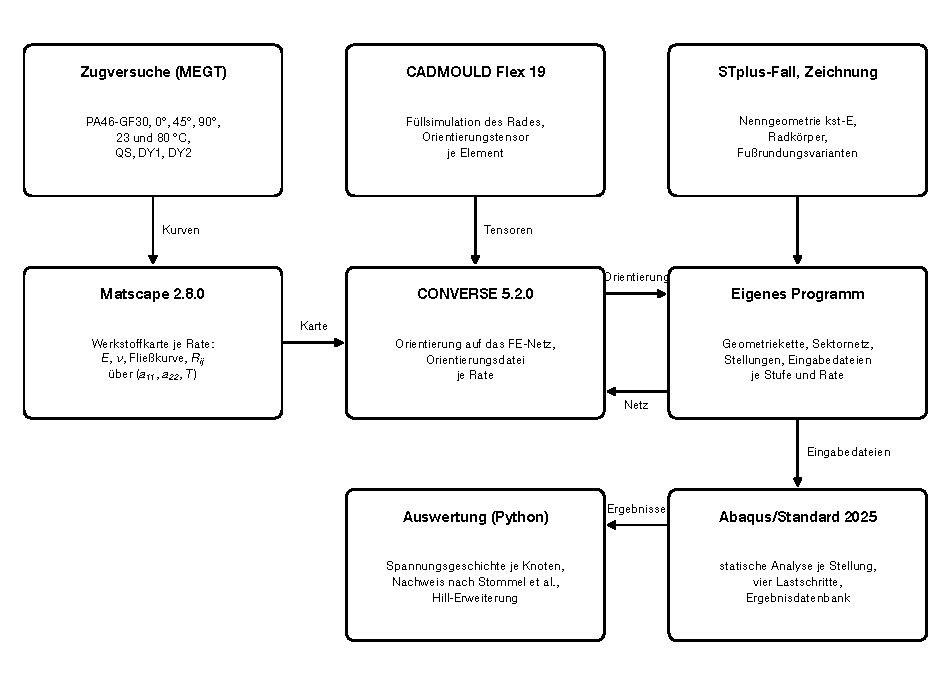
\includegraphics[width=0.95\textwidth]{kap3/flussbild_kette}
	\caption{Simulationskette von den Zugversuchen zum Nachweis: Programme als Kästen, die übergebenen Daten an den Pfeilen.}
	\label{fig:flussbild_kette}
\end{figure}

Die Zugversuche wurden am Lehrstuhl für Maschinenelemente, Getriebe und Tribologie (MEGT) der Rheinland-Pfälzischen Technischen Universität Kaiserslautern-Landau durchgeführt. Werkstoff war das konditionierte PA46-GF30 Stanyl TW200F6 von Envalior, geprüft bei $23$ und $80$\,\textdegree C an Proben unter $0$\textdegree, $45$\textdegree{} und $90$\textdegree{} und bei drei Prüfgeschwindigkeiten. Der quasistatischen Karte QS liegen die Richtungen $0$\textdegree{} und $90$\textdegree{} zugrunde, den dynamischen Karten DY1 und DY2 alle drei Richtungen. Matscape 2.8.0 von PART Engineering passt an diese Kurven je Prüfgeschwindigkeit eine Werkstoffkarte an. Sie enthält die elastischen Konstanten als Gitter über dem Orientierungszustand und der Temperatur. Der Zustand wird durch die beiden größten Eigenwerte $a_{11}$ und $a_{22}$ des Orientierungstensors beschrieben. Dazu kommen die Fließkurve des $0$\textdegree-Stabes als wahre Spannung und die Fließspannungsverhältnisse nach Hill je Orientierungszustand. Die Versagensart stuft Matscape aus den Versuchsdaten als duktil ein.

Die Faserorientierung stammt aus einer Spritzgießsimulation des Rades mit Cadmould Flex 19.0.1.10 in der Strategie 3D-F mit einer Elementkante von $1$\,mm. Das reale Werkzeug mit dem Stahleinleger und dem später abgetrennten Zentralanguss stand nicht zur Verfügung. Ein virtueller Verteiler mit 238 Anspritzpunkten auf den Radien $15{,}0$ bis $19{,}1$\,mm in der Stegebene füllt deshalb das Bauteil. \tabref{tab:cadmould} nennt die Prozessparameter des Laufs. Das Orientierungsergebnis liegt als binäre Datei vor, die hier nicht gelesen wird. In die Kette geht es allein über CONVERSE ein.

\begin{table}[htbp]
	\caption{Einstellungen der Spritzgießsimulation des Rades in CADMOULD.}
	\label{tab:cadmould}
	\centering
	\small
	\begin{tabular}{ll}
		\hline
		Größe                            & Wert                                                                       \\
		\hline
		\arrayrulecolor{black!30}
		Programm und Strategie           & Cadmould Flex 19.0.1.10, 3D-F                                              \\
		\hline
		Elementkante in mm               & $1$                                                                        \\
		\hline
		Werkstoff                        & Stanyl TW200F6 (Envalior)                                                  \\
		\hline
		Faserfaktoren                    & $0{,}99$; $0{,}94$; $0{,}09$                                               \\
		\hline
		Interaktionskoeffizient          & $0{,}01$                                                                   \\
		\hline
		Anspritzung                      & virtueller Verteiler, 238 Punkte, $r$ $15{,}0$ bis $19{,}1$\,mm, Stegebene \\
		\hline
		Füllzeit in s                    & $0{,}554$                                                                  \\
		\hline
		Massetemperatur in \textdegree C & $315$                                                                      \\
		\hline
		Wandtemperatur in \textdegree C  & $100$                                                                      \\
		\hline
		Nachdruck in bar, Dauer in s     & $500$; $10{,}9$                                                            \\
		\arrayrulecolor{black}
		\hline
	\end{tabular}
\end{table}

CONVERSE 5.2.0 überträgt das Orientierungsergebnis auf das Netz des FE-Modells. Die Ausgabe ist eine Orientierungsdatei im Abaqus-Format. Sie enthält je Element das Faserkoordinatensystem als Verteilung, je Knoten die Eigenwerte $a_{11}$ und $a_{22}$ als Feldvariablen und die Werkstoffkarte der Rate. Für jede Rate entsteht eine Datei. Die Orientierungszeilen der drei Dateien sind gleich, nur die Werkstofftabellen unterscheiden sich. Da die Elementnummern jedes Netzes eigen sind, braucht jeder Körper und jede Fußrundungsvariante ein eigenes CONVERSE-Mapping. Vor dem Schreiben der Eingabedateien wird geprüft, dass Element- und Knotennummern der Orientierungsdatei genau die des Netzes sind und der Name der Karte zur Rate passt. Der Sektor liegt in jedem CONVERSE-Mapping an derselben Winkelstellung des Rades, weil das Spritzgießergebnis nicht rotationssymmetrisch ist (vgl. \secref{sec:faserorientierung}).

Netz und Eingabedateien erzeugt das in \secref{sec:werkzeugkette} beschriebene Programm. Es baut den Sektor aus der erzeugten Zahnkontur und dem Radkörper der Zeichnung und schreibt je Stellung, Werkstoffstufe und Rate eine Eingabedatei. Die Orientierungsdatei wird dafür in einen Teil für das Bauteil und einen Teil für das Modell zerlegt. Der Elementsatz ihrer Querschnittsdefinition wird auf den des Netzes umgeschrieben. Eine Manifestdatei je Ordner hält Netz, Stellungen, Momente, Karten und Lösereinstellungen fest (vgl. \anhref{sec:anhang_c}).

Gerechnet wird mit Abaqus/Standard 2025 auf einer Vollversion mit vier Kernen. Funktionstests kleiner Modelle liefen in der Learning Edition. Die Ergebnisdatenbanken werden nach \secref{sec:auswertung_beanspruchung} ausgelesen und bleiben erhalten, so dass weitere Größen nachträglich gelesen werden können.

Neben Abaqus dient ein eigener ebener Löser der Konvergenzstudie und der ebenen Fußrundungsstudie (\secref{sec:netzkonvergenz}, \secref{sec:werkzeugkette}). Er rechnet den Stirnschnitt des Sektors im ebenen Dehnungszustand linear elastisch, isotrop und mit kleinen Verschiebungen. Das Vierknotenelement liegt in zwei Formulierungen vor, selektiv reduziert integriert wie CPE4 und C3D8 sowie mit inkompatiblen Moden wie CPE4I und C3D8I. Die Spannungen werden wie in Abaqus von den Gaußpunkten auf die Knoten extrapoliert und gemittelt. Am Einzahnsektor mit 859 Knoten stimmt er mit Abaqus in der Learning Edition auf $7 \cdot 10^{-5}$ überein.

Die Paarung wird ausschließlich in Abaqus gerechnet. Ein eigenes Modell wurde aufgebaut, weil die FVA-Workbench als geschlossenes Werkzeug Konvergenzstudien über mehrere Netze nur bedingt zulässt. Zudem sollte die vollständige Kette skriptbasiert in Python umgesetzt werden, um diese Art der Programmierung zu erlernen. Nachträglich geänderte Eingabedateien der Workbench konvergierten bei werkstofflicher und geometrischer Nichtlinearität außerdem schlecht. Das Netz der Verzahnung kst-E, mit dem die Zahnfußspannung dort ausreichend aufgelöst ist, dient als Ausgangsdiskretisierung.

\subsection{Aufbau des Modells}
\label{sec:fe_modellaufbau}

Das Rad wird als Sektor aus fünf Zähnen mit je einem zahnlosen Teilungsabschnitt an beiden Enden modelliert. Die Topologie des Stirnschnitts stammt von einem Referenzmodell der FVA Workbench zur Verzahnung kst-E \cite{FVA856-I}, dessen Schnitt entlang der Lückenmitten in einen Schulterblock und kongruente Zahnblöcke zerfällt. Auf die erzeugte Kontur werden die Oberflächenknoten stückweise gesetzt, so dass Fußformpunkt, Kopfformpunkt und Kopfecke Knoten sind. Das Innere folgt durch harmonische Fortsetzung der Oberflächenverschiebung. \figref{fig:netz_sektor} zeigt den Sektor, \figref{fig:netz_zahn} den Stirnschnitt eines Zahns mit der Randschicht an Flanke und Fußrundung.

% TK erledigt (Grid über plot_style axes.axisbelow in allen Bildern nach hinten): Hier in dem Bild fällt es richtig auf, dass das Grid über den eigentlich zu sehenden Bild ist. Das Grid soll aber immer in der hintersten Ebene liegen, dass es das geezigt nicht überlappt. Bitte auch nochmal bei anderen Bildern überprüfen. Bild 3.5 ist beispielsweise korrekt.

\begin{figure}[htbp]
	\centering
	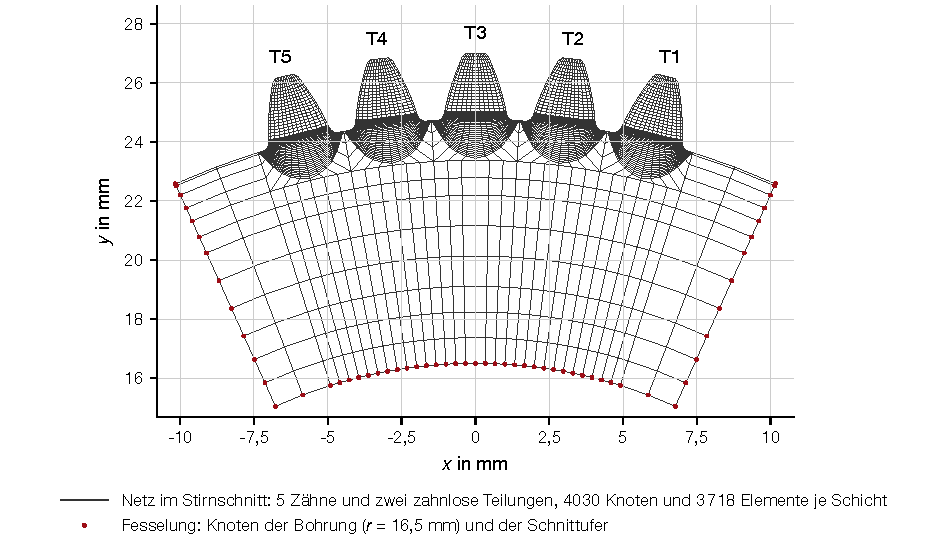
\includegraphics[width=0.7\textwidth]{kap3/netz_sektor}
	\caption{Sektornetz des Rades mit Taschenkörper, 20 Schichten über der Zahnbreite, Bohrung $33$\,mm.}
	\label{fig:netz_sektor}
\end{figure}

\begin{figure}[htbp]
	\centering
	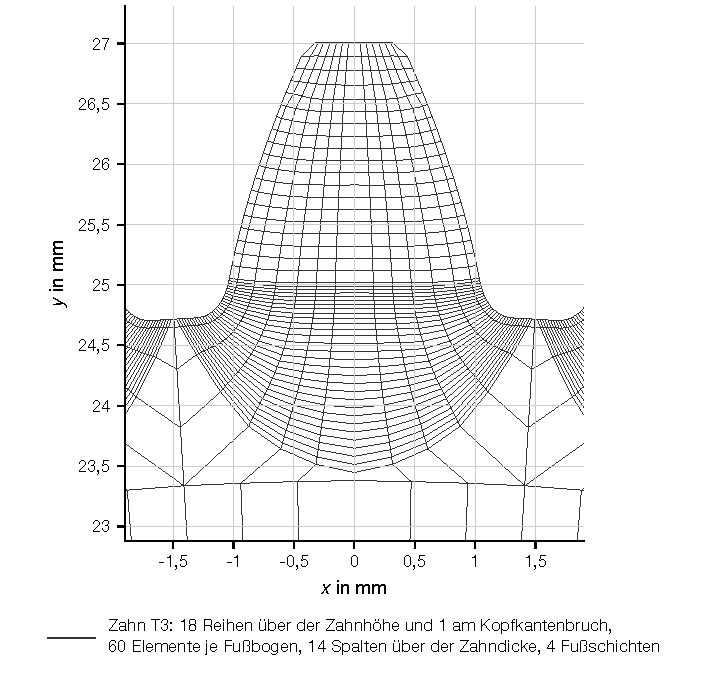
\includegraphics[width=0.7\textwidth]{kap3/netz_zahn}
	\caption{Netz eines Zahns im Stirnschnitt: Randschicht an Flanke und Fußrundung, Vergröberung zum Körper.}
	\label{fig:netz_zahn}
\end{figure}

Die Diskretisierung folgt der Konvergenzstudie am ebenen Sektor in \secref{sec:netzkonvergenz}. Sie ist je Bereich des Zahns verschieden fein. Über der Zahnhöhe liegen 18 Elementreihen und eine am Kopfkantenbruch, am Fußbogen 60 je Lücke, über der Zahndicke 14, dazu vier Fußschichten normal zur Fußoberfläche und zwei Spalten je Schulter. In Richtung der Zahnbreite von $15$\,mm liegen 20 Schichten. Dieses Netz ist die Grundlage jedes CONVERSE-Mappings der Faserorientierung.

Der Radkörper folgt der überbemaßten Zeichnung des Rades (vgl. \anhref{sec:anhang_a}). Die Nabe reicht in voller Breite von der Bohrung mit dem Radius $16{,}5$\,mm bis zum Radius $19{,}107$\,mm. Von beiden Stirnseiten ist je eine Tasche bis zum Radius $22{,}168$\,mm eingeformt, $5{,}5$\,mm tief, mit Wänden unter $93$\textdegree{} zur Stirnseite. Zwischen den Taschen bleibt ein Steg von $4$\,mm, vergleichbar mit einem I-Profil in voller Breite der Zähne. Die Rundungen R\,$0{,}5$ der Zeichnung sind nicht vernetzt. Das Stirnschnittnetz behält seine Zahnzone. Die Ringe des I-Profils werden Schicht für Schicht auf Bohrung, Nabenwand und Profilwand gelegt, wobei die Formschräge der Wände mitgeht. Die Elemente innerhalb der Taschen werden entfernt. Das I-Profil erhält acht Ringe, der Steg sechs Schichten und jede Tasche sieben. Der Taschenkörper hat damit 83\,650 Knoten und 72\,932 Elemente (vgl. \figref{fig:netz_koerper}). Der Vollring mit Bohrung, der Bezugskörper der Netzstudien in \chapref{chap:voruntersuchungen}, wird dort auf derselben Schichtung wie der Taschenkörper geführt und hat 82\,425 Knoten und 72\,320 Elemente. Er trägt trotz des vollen Querschnitts weniger Elemente, weil er radial nur fünf Kranzringe hat.

% TK erledigt (Zahlen des Rings auf Taschenschichtung, Grund: fünf gegen acht Ringe): Warum hat der Vollring weniger Elemente und Knoten als der Taschenkörper. Das hatten wir doch geklärt, dass wir den Vollring dann nur noch mit dem angepassten mesh vom I-Profilkörper verwednen. Bitte von dem die Werte dort im Text einsetzen.

\begin{figure}[htbp]
	\centering
	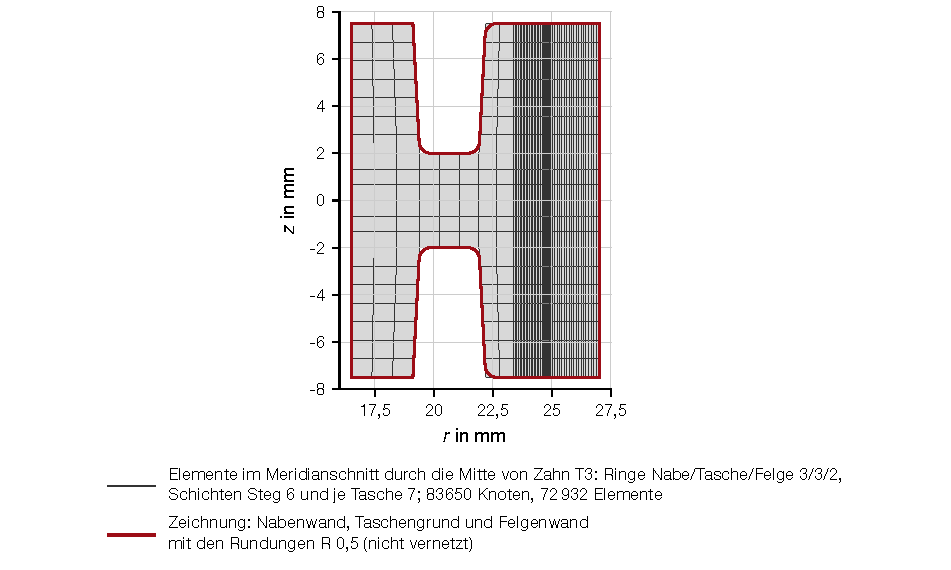
\includegraphics[width=0.7\textwidth]{kap3/netz_koerper}
	\caption{Radkörper nach Zeichnung: Nabe, Steg und Taschen mit Formschräge.}
	\label{fig:netz_koerper}
\end{figure}

% TK erledigt (Bild in 3.1 gestrichen, hier mit z horizontal neu): Das Bild gibt es schonmal. Hier deutlich aufgeräumter. Die ganzen Bezeichnungen an der anderen Stelle braucht es nicht. Bitte nur hier einbinden und nicht an der ersten Stelle. DAs reicht. Dennoch wie in der anderen Markierung genannt die z-Achse auf die Horizontale legen, dass kann ess sich der LEser besser Vorstellen und verstehte die Bezeichnung I-Profil über den Umfang.

Der Stahleinleger des realen Rades sitzt in der Bohrung mit $33$\,mm Durchmesser. Er wird nicht vernetzt, sondern als starre Fesselung abgebildet. Bohrungsknoten und beide Schnittflächen des Sektors sind als starrer Körper an den Bezugspunkt des Rades gebunden, der in allen Freiheitsgraden festgehalten ist. Weil die festen Schnittflächen auf die äußeren Zähne zurückwirken, wird der mittlere Zahn T3 ausgewertet.

Das Stahlritzel geht nur mit seiner Zahnoberfläche in das Modell ein, als starre Fläche aus vierknotigen Elementen R3D4 mit Facetten bis $0{,}05$\,mm Kantenlänge, ohne Volumen, Stirnflächen und Werkstoff. Sie umfasst sieben Zähne und ist an einen Bezugspunkt auf der Ritzelachse gebunden, der Drehung und Moment aufnimmt. Dass das Ritzel als starre Fläche modelliert wird, folgt aus der Paarung Stahl gegen Kunststoff. Die Kopfkanten des Ritzels sind in dieser Fläche gerundet, mit $0{,}1$\,mm und zwölf Facetten je Bogen. Das reale Ritzel hat nach Zeichnung und Konturscan eine scharfe Kante. Die Rundung ist eine Entscheidung des Modells, die in \secref{sec:kopfkante} aus den Abbrüchen an der scharfen Kante begründet und in ihrem Einfluss untersucht wird. \figref{fig:paarung_netz} zeigt Sektor und Ritzelfläche in der Rechenlage im Normpunkt C.

\begin{figure}[htbp]
	\centering
	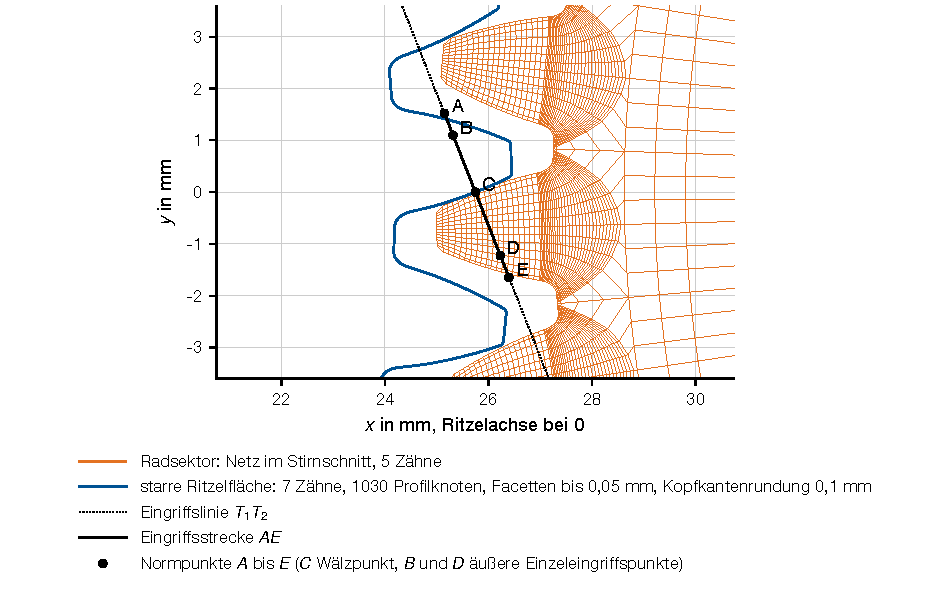
\includegraphics[width=0.7\textwidth]{kap3/paarung_netz}
	\caption{Radsektor und starre Ritzelfläche in der Stellung C mit Eingriffslinie und den Normpunkten A bis E.}
	\label{fig:paarung_netz}
\end{figure}

% TK erledigt (Grid nach hinten): Auch hier das Grid in der vordersten und nicht hintersten Ebene. Wie, wenn man auf einem Karierten Papier schreibt musst du dir vorstellen. Da überdeckt die Tinte auch den Blatthintergrund. Deswgen Grid nach hinten.

Die Lage des Paares wird je Stellung analytisch aus der Evolventengeometrie bestimmt. Eine einzige Größe, der Krümmungsradius der Ritzelflanke im Berührpunkt des verfolgten Zahnpaares, legt beide Räder fest. Die Arbeitsflanken berühren sich, das gesamte Flankenspiel liegt an den Rückflanken. Der Drehsinn ist der des Prüfstands. Bei Blick auf die Stirnseite mit dem Ritzel links dreht das treibende Ritzel im Uhrzeigersinn, und die rechten Flanken arbeiten. Beide Räder sind als Bauteile mit festen Achsen definiert und werden je Stellung als Instanzen verschoben und um ihre Achsen gedreht. Eine am Bauteil definierte Orientierung dreht in Abaqus mit der Instanz mit, auch wenn sie als Verteilung vorliegt, so dass die Faserorientierung dem Rad in jede Stellung folgt. Bei jedem Lauf mit Orientierungsdatei wird dies an den lokalen Werkstoffrichtungen der Ergebnisdatenbank geprüft.

Der Kontakt ist als Knoten-zu-Fläche-Paar mit der Radflanke als Nebenfläche und der starren Ritzelfläche als Hauptfläche definiert. Die Normalen der facettierten starren Fläche werden mit dem Glättungsmaß $0{,}2$ geglättet, so dass die Kontaktkraft normal zur Ritzelflanke bleibt. Die Kontaktbedingung ist hart und reibungsfrei und wird mit Lagrange-Multiplikatoren erzwungen, der Voreinstellung von Abaqus für diese Formulierung. Stabilisierung, Dämpfung und Masse sind ausgeschlossen. Die Lösereinstellungen und Iterationsgrenzen stehen in \anhref{sec:anhang_c}. Die Wahl der Kontaktformulierung wird in \secref{sec:kopfkante} begründet.

% TK erledigt (Pilotergebnisse zu Iterationsgrenzen und Fläche-zu-Fläche gestrichen; ebenso gestrichen: 40/80-Schichten-Piloten im Netzabsatz, NLGEOM-Prozente und C3D8I-Abbrüche im Stufenabsatz, alle mit Verweis auf 4.1): Der Abschnitt greift schon zu sehr dem Kapitel 4 vor, wo die Netzkonvergenz durchprobiert wurde. Bitte rausnehmen. Ich mache es bewusst nicht manuell, dass du den Fehler merkst und auch bei anderen Abschnitten Kürzungen vorschlägst, die thematisch einem anderen Kapitel/Abschnitt gehören.

Jede Rechnung ist eine implizite statische Analyse mit vier Schritten. Im ersten Schritt wird dem Ritzel eine Drehung um einen Bogen von $1$\,\textmu m am Grundkreis vorgegeben, die den Kontakt schließt. Danach folgen drei statische Schritte, in denen die Vorgabe entfällt und das Moment als Last auf den Drehfreiheitsgrad des Ritzels wirkt. Die Momente am Rad betragen $8$, $12$ und $16$\,Nm wie im Laufversuch und werden am Ritzel mit
\begin{equation}
	T_1 = T_2 \, \frac{z_1}{z_2}
	\label{eq:moment_ritzel}
\end{equation}
aufgebracht, dem Betrag nach $7846$, $11\,769$ und $15\,692$\,Nmm. Das Vorzeichen folgt dem Drehsinn des Prüfstands, so dass das treibende Ritzel die Arbeitsflanke des Rades belastet. Das Ritzel dreht sich unter dem Moment bis zum Gleichgewicht. Nichts wälzt innerhalb einer Analyse ab. Dieser Verdrehwinkel des Ritzels bis zum Gleichgewicht ist in den folgenden Kapiteln das Maß der Verformung. Er enthält die Biegung der Radzähne und die Nachgiebigkeit des Kontakts, nicht das Flankenspiel, weil die Arbeitsflanken zu Beginn jeder Rechnung berühren. Je Schritt werden Spannungen, Dehnungen, Verschiebungen und Kontaktgrößen in die Ergebnisdatenbank geschrieben, dazu Kräfte, Stützmoment und Drehung beider Bezugspunkte in die Textausgabe.

% TK erledigt (Moment als Betrag mit Drehsinn des Prüfstands; Verdrehwinkel definiert): Drehsinn mit im Uhrzeigersinn vom Text und x y aus den Bildern würde bei der Angabe eines positiven Moment gegen Uhrzeigersinn nach rechter Hand und Daumenregel drehen. Bitte entweder Betrag einbinden oder anders formulieren.

Die Eingriffsstrecke wird nicht in einer Abwälzsimulation durchlaufen, sondern in Einzelstellungen. Nach Stommel et al. \cite[S.~56 bis 57]{Sto18} sind elastisch-plastische Werkstoffmodelle für Kunststoffe nur unter monotoner Belastung sinnvoll. Ein an der Spannungs-Dehnungs-Kurve kalibriertes Modell zählt viskoelastische Dehnung als plastische und weist die bleibende Dehnung zu groß aus. Ein Abwälzen be- und entlastet jeden Zahn, und die Lastgeschichte, die es mitführen würde, bestünde aus genau diesen Dehnungen. Die Erstbelastung je Stellung ist die Belastung, für die das Modell gilt. Für elastischen Werkstoff führen beide Wege zum gleichen Zustand, so dass das Abwälzen in einer Simulation als Gegenprobe mit elastischem Werkstoff dem Ausblick vorbehalten bleibt (vgl. \secref{sec:ausblick}).

% TK erledigt (S. 56 bis 57; alle Zitate ohne Seite werden in Paket A3 nachgezogen): Zitat nur noch ohne Seite. Entweder in der gesamten Arbeit mit Seitenzahlen beim zitieren arbeiten oder gar nicht. Bitte einheitlich. Gerne mit Seitenzahlen.

Die Stellungen liegen auf einem Gitter über dem Eingriffsweg mit 30 Stellungen je Eingriffsteilung, von einer Teilung vor dem Eingriffsbeginn A bis eine Teilung nach dem Eingriffsende E. Zusätzlich werden die Normpunkte A bis E als eigene Stellungen gerechnet. Die äußeren Einzeleingriffspunkte B und D folgen DIN ISO 21771 \cite{DINISO21771}. Mit $p_{\mathrm{bt}} = 2{,}952$\,mm und $g_{\alpha} = 3{,}406$\,mm ergibt das 99 Stellungen je Serie. Der Rand von einer Teilung deckt den durch die Verformung verlängerten Eingriff ab. Gitterweite und Rand wurden in den Voruntersuchungen festgelegt (vgl. \chapref{chap:voruntersuchungen}). Die Lage des Paares in der Stellung C mit der Eingriffsstrecke zeigt \figref{fig:paarung_netz}.

\subsection{Werkstoffstufen und Dehnraten}
\label{sec:werkstoffstufen}

Der Werkstoff des Rades wird in vier Stufen beschrieben, die alle auf derselben Karte beruhen und außerhalb der Werkstoff- und Querschnittsblöcke gleiche Eingabedateien haben (vgl. \tabref{tab:werkstoffstufen}). W1 nimmt die isotrope Zeile der Karte bei $80$\,\textdegree C als linear elastischen Werkstoff. W2 ergänzt sie um die Fließkurve und die Fließspannungsverhältnisse nach Hill derselben Zeile. Da Abaqus anisotrope Fließbedingungen nur in einem lokalen System zulässt, trägt W2 das Bauteilsystem als Orientierung. W3 verwendet die Orientierungsdatei ohne Plastizität, die elastischen Konstanten folgen dann je Element dem Orientierungszustand des CONVERSE-Mappings. W4 verwendet die vollständige Orientierungsdatei.

Elementtyp und Kinematik richten sich nach der Stufe. Die elastischen Stufen W1 und W3 werden geometrisch linear mit C3D8I, dem Element mit inkompatiblen Moden, gerechnet. Die elastisch-plastischen Stufen W2 und W4 werden geometrisch nichtlinear mit C3D8, dem Element mit selektiv reduzierter Integration, auf demselben Netz gerechnet. Die nichtlineare Rechnung ist gewählt, weil die Fließkurve der Karte bei $80$\,\textdegree C schon bei $4{,}3$\,MPa beginnt und Stommel et al. für Kontakt und große Verformung den nichtlinearen Löser vorsehen \cite[S.~474]{Sto18}. Die Gründe für diese Zuordnung, die Abbrüche von C3D8I unter geometrischer Nichtlinearität und das Konvergenzverhalten beider Elemente stehen in \secref{sec:netzkonvergenz}. Fußspannungen werden nur innerhalb eines Elementtyps verglichen.

\begin{table}[htbp]
	\caption{Werkstoffstufen des FE-Modells, Datenquelle, Elementtyp und Kinematik.}
	\label{tab:werkstoffstufen}
	\centering
	\small
	\begin{tabular}{lL{4.2cm}L{4.8cm}ll}
		\hline
		Stufe & Werkstoffmodell                & Datenquelle                         & Element & NLGEOM \\
		\hline
		\arrayrulecolor{black!30}
		W1    & isotrop, linear elastisch      & isotrope Zeile der Karte            & C3D8I   & nein   \\
		\hline
		W2    & isotrop, elastisch-plastisch   & isotrope Zeile, Fließkurve, Hill    & C3D8    & ja     \\
		\hline
		W3    & anisotrop, elastisch           & Orientierungsdatei ohne Plastizität & C3D8I   & nein   \\
		\hline
		W4    & anisotrop, elastisch-plastisch & vollständige Orientierungsdatei     & C3D8    & ja     \\
		\arrayrulecolor{black}
		\hline
	\end{tabular}
\end{table}

Die drei Karten unterscheiden sich in der Prüfgeschwindigkeit der zugrunde liegenden Zugversuche (vgl. \tabref{tab:raten}). Die Steifigkeit wächst mit der Dehnrate. Jede Werkstoffstufe wird mit jeder Rate gerechnet. W1 und W2 nehmen die isotrope Zeile der Karte ihrer Rate, so dass die Ratenachse für alle vier Stufen gilt. Alle Karten werden bei $80$\,\textdegree C ausgewertet, weil die Laufversuche auf diese Zahnmassentemperatur geregelt sind (\secref{sec:pruefstand}, \secref{sec:temperatur}).

In \figref{fig:orientierungszustaende_qs} stehen die gemessenen Kurven in und quer zur Fließrichtung neben den Kurven dreier Orientierungszustände der quasistatischen Karte. Jede Zustandskurve entsteht aus der Referenzkurve in Fließrichtung durch Skalieren mit dem Fließspannungsverhältnis und dem Modul des Zustands. Der Zustand des Zahnfußes ist der Orientierungszustand, den das CONVERSE-Mapping am Fuß des Zahns T3 liefert, mit den Eigenwerten $a_{11} = 0{,}64$ und $a_{22} = 0{,}083$. Die Orientierungsdateien tragen je Element diesen Tensor, die Karte das Kennwertgitter, aus dem die Kurve des Zustands interpoliert wird. Der isotrope Zustand liegt nahe der Messung quer zur Fließrichtung. Das erklärt sich daraus, dass ein regellos orientierter Kurzfaserverbund in jeder Richtung nur einen kleinen Teil der Faserwirkung trägt. Die Probe quer zur Fließrichtung aus einem hochorientierten Stab besitzt dagegen noch Restverstärkung. Der ausgerichtete Zustand liegt deutlich über der Messung in Fließrichtung, und der stark ausgerichtete Fußzustand trifft annähernd die Messung in Fließrichtung.

\begin{figure}[htbp]
	\centering
	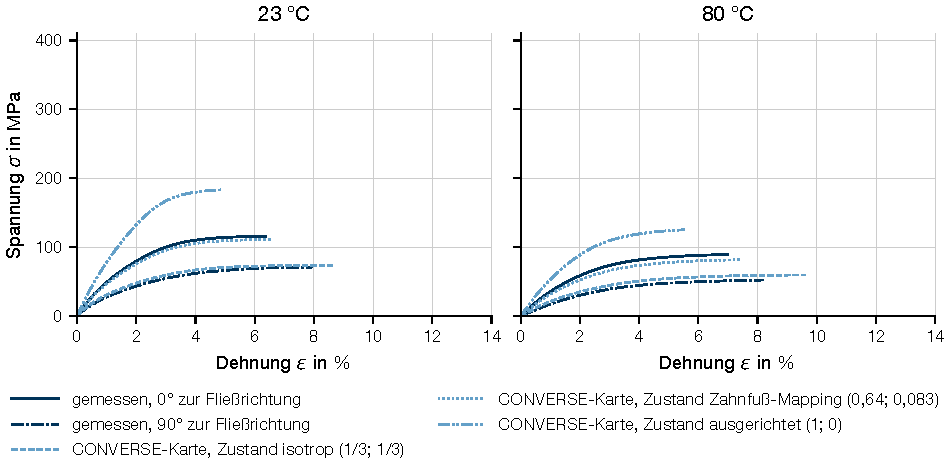
\includegraphics[width=0.95\textwidth]{kap2/orientierungszustaende_qs}
	\caption{Gemessene Richtungen und Orientierungszustände der quasistatischen Werkstoffkarte von PA46-GF30 bei $23$ und $80$\,\textdegree C (Matscape-Karte, Zustandskurven aus der Referenzkurve in Fließrichtung mit $R_{\mathrm{11}}$ und $E_{\mathrm{1}}$ des Zustands).}
	\label{fig:orientierungszustaende_qs}
\end{figure}

\begin{table}[htbp]
	\caption{Werkstoffkarten der drei Dehnraten. $E$ und $\nu$ aus der isotropen Zeile jeder Karte bei $80$\,\textdegree C.}
	\label{tab:raten}
	\centering
	\small
	\begin{tabular}{llllll}
		\hline
		Karte & Prüfgeschwindigkeit in m/s & Dehnrate in 1/s             & $E$ in MPa  & $\nu$      & Temperatur in \textdegree C \\
		\hline
		\arrayrulecolor{black!30}
		QS    & $0{,}0000167$              & $0{,}00027$ bis $0{,}00044$ & $2282{,}08$ & $0{,}2997$ & $80$                        \\
		\hline
		DY1   & $0{,}174$                  & $3$                         & $2542{,}51$ & $0{,}2951$ & $80$                        \\
		\hline
		DY2   & $10$                       & $60$                        & $3596{,}61$ & $0{,}2973$ & $80$                        \\
		\arrayrulecolor{black}
		\hline
	\end{tabular}
\end{table}

Welche Karte dem Prüfstand am nächsten kommt, folgt aus der Dehnungsgeschichte des Zahnfußes im Modell. Bei $3000$\,1/min am Rad läuft der Berührpunkt mit $7{,}7$\,m/s über die Eingriffslinie, eine Teilung in $0{,}385$\,ms, und die Zugspannung der Fußrundung steigt vom Eintritt des Zahns bis zu ihrem Größtwert über rund $3{,}2$\,mm Wälzweg, also in $0{,}42$\,ms, auf $2{,}6$ bis $3{,}8$\,\% Dehnung der Stufe W1. Das ergibt je Stufe einen Wert, $60$\,1/s bei $8$\,Nm und $90$\,1/s bei $16$\,Nm mit dem Modul der quasistatischen Karte und $45$ beziehungsweise $70$\,1/s mit dem Modul der Karte DY2, bei $2250$\,1/min jeweils drei Viertel davon (\secref{sec:stufen_raten_koerper}). Die Karte DY2 mit $60$\,1/s liegt dem Prüfstand damit am nächsten, QS ist die untere Grenze.

% TK erledigt (Nullen ergänzt, Ursache: latexindent 4.0 entfernt die 0 nach einem Dollarzeichen; Satz zur Karte der Belastungsgeschwindigkeit ergänzt): In der Tabelle werden die 0 en vor dem Komma angezeigt in anderern Tabellen und manchmal im Text nicht. Bitte die 0 vor dem Komma überall geränzen. Vielleicht noch einen Satz erwähnen, welche Karte der realen Belastungsgeschwindigkeit am nähsten kommt, wenn es nicht an anderer Stelle erwähnt wird.

Als zweite Werkstoffquelle der anisotropen elastischen Stufe dienen die elastischen Konstanten der konditionierten Randschicht aus Tabelle~4 des Abschlussberichts FVA 856 I \cite{FVA856-I} (vgl. \tabref{tab:fva856_tab4}). Der Bericht hat sie aus Zugversuchen an $0$\textdegree- und $90$\textdegree-Proben mit einer mikromechanischen Zelle umgerechnet. In dieser Variante ersetzt der Block mit den neun Konstanten bei $80$\,\textdegree C und der jeweiligen Rate den orientierungsabhängigen Elastizitätsblock der Karte. Die Konstanten gelten unverändert über dem ganzen Rad im Faserkoordinatensystem, das das CONVERSE-Mapping je Element vorgibt. Die Richtung 1 ist die Faservorzugsrichtung. Daneben wurde eine zweite Richtungsquelle aufgebaut, in der die Zonenkarte der CT-Befunde des Berichts den fünf Zähnen des Sektors zugewiesen wird. Werkstoffquelle und Richtungsquelle werden so in einem Schema aus zwei mal zwei Varianten getrennt (vgl. \secref{sec:faserorientierung}).

\begin{table}[htbp]
	\caption{Elastische Konstanten der konditionierten Randschicht von PA46-GF30 bei $80$\,\textdegree C nach Tabelle~4 des Berichts FVA 856 I. Richtung 1 Faservorzugsrichtung.}
	\label{tab:fva856_tab4}
	\centering
	\small
	\begin{tabular}{llllllllll}
		\hline
		Karte & $E_{1}$ & $E_{2}$ & $E_{3}$ & $\nu_{12}$ & $\nu_{13}$ & $\nu_{23}$ & $G_{12}$ & $G_{13}$ & $G_{23}$ \\
		      & MPa     & MPa     & MPa     &            &            &            & MPa      & MPa      & MPa      \\
		\hline
		\arrayrulecolor{black!30}
		QS    & $4156$  & $1444$  & $1369$  & $0{,}423$  & $0{,}386$  & $0{,}495$  & $683$    & $585$    & $469$    \\
		\hline
		DY1   & $4823$  & $1866$  & $1790$  & $0{,}416$  & $0{,}384$  & $0{,}495$  & $845$    & $739$    & $611$    \\
		\hline
		DY2   & $6193$  & $2931$  & $2861$  & $0{,}404$  & $0{,}380$  & $0{,}489$  & $1241$   & $1124$   & $974$    \\
		\arrayrulecolor{black}
		\hline
	\end{tabular}
\end{table}

Die Fußrundungsvarianten aus \secref{sec:werkzeugkette} gehen als Netzvarianten ein. Die Sektorvorlage wird auf die neue Kontur abgebildet, Ritzelfläche, Körper und Lasten bleiben gleich.

\subsection{Umfang der Rechnungen}
\label{sec:rechenumfang}

\tabref{tab:rechenumfang} fasst die gerechneten Serien und Piloten zusammen. Serien laufen über das volle Stellungsgitter, Piloten über die fünf Normpunkte. Die Auflösungsstudie mit 60 Stellungen je Teilung und scharfer Ritzelkante ging dem Gitter der Serien voraus. Auf der Vollversion mit vier Kernen braucht eine Stellung des Ringkörpers im Mittel $3{,}8$\,min in W1, $5{,}0$\,min in W2, $8{,}7$\,min in W3 und $12{,}6$\,min in W4. Der Taschenkörper lag in seinem Piloten bei $3{,}4$ bis $10{,}7$\,min. Die Serie der gefertigten Paarung lief mit drei Jobs zu je vier Kernen auf zwölf Kernen in $77{,}6$\,h, die Serie der bionischen Fußrundung wurde nach den Normpunkten abgebrochen.

\begin{table}[htbp]
	\caption{Gerechnete Serien und Piloten. Jobs sind Eingabedateien je Stellung, Werkstoffstufe und Rate. Zeiten aus dem Simulationstagebuch, k.\,A. dort nicht als Summe erfasst.}
	\label{tab:rechenumfang}
	\centering
	\footnotesize
	\begin{tabular}{L{4.0cm}lllL{1.6cm}lL{2.0cm}}
		\hline
		Rechnung                                                                       & Körper & Stufen    & Raten        & Stellungen & Jobs          & Zeit                                       \\
		\hline
		\arrayrulecolor{black!30}
		Auflösungsstudie, 60 je Teilung, Kante scharf                                  & Ring   & W1        & QS           & 133        & 133           & rund $10$\,h                               \\
		\hline
		Serie, 30 je Teilung, Rand 1 Teilung                                           & Ring   & W1 bis W4 & QS           & 99         & 396           & $50{,}0$\,h                                \\
		\hline
		Ratenpilot                                                                     & Ring   & W1 bis W4 & DY1, DY2     & A bis E    & 40            & k.\,A.                                     \\
		\hline
		Pilot Taschenkörper                                                            & Tasche & W1 bis W4 & QS, DY1, DY2 & A bis E    & 60            & $6{,}5$\,h                                 \\
		\hline
		Pilot Ring auf Taschenschichten                                                & Ring   & W1 bis W4 & QS, DY1, DY2 & A bis E    & 60            & $6{,}0$\,h                                 \\
		\hline
		Pilot CT-Zonen-Orientierung                                                    & Ring   & W3, W4    & QS, DY1, DY2 & A bis E    & 30            & $4{,}8$\,h                                 \\
		\hline
		Piloten Tabelle~4, CONVERSE-Mapping und CT-Zonen                               & Ring   & W3        & QS, DY1, DY2 & A bis E    & 2 $\times$ 15 & k.\,A.                                     \\
		\hline
		Piloten Kopfkontakt, 36 und 54 Reihen, Kante $0{,}1$ / $0{,}05$ / $0{,}02$\,mm & Ring   & W1, W2    & QS           & A bis E    & 40            & k.\,A.                                     \\
		\hline
		Fußrundungsvarianten, sechs Konturen                                           & Tasche & W1 bis W4 & QS, DY1, DY2 & A bis E    & 6 $\times$ 60 & $7{,}8$ bis $8{,}9$\,h je Variante         \\
		\hline
		Serie Taschenkörper                                                            & Tasche & W1 bis W4 & QS           & 99         & 396           & gerechnet, 387 vollständig                 \\
		\hline
		Serie bionische Fußrundung                                                     & Tasche & W1 bis W4 & QS           & 99         & 396           & abgebrochen, A bis E gerechnet             \\
		\hline
		Serie gefertigte Paarung, Kopfkappe                                            & Tasche & W1 bis W4 & QS, DY1, DY2 & 99         & 1188          & $77{,}6$\,h, drei Jobs parallel            \\
		\hline
		Piloten Ritzel und Rad einzeln wie gefertigt                                   & Tasche & W1 bis W4 & QS, DY1, DY2 & A bis E    & 2 $\times$ 60 & $3{,}7$ und $4{,}1$\,h, drei Jobs parallel \\
		\arrayrulecolor{black}
		\hline
	\end{tabular}
\end{table}

% Bildwunsch: Flussbild der Simulationskette (T6, eigene Zeichnung), Zugversuche bis Auswertung mit den Dateiformaten je Glied.
% Bildwunsch: 80_output/fe/kst_e/bilder_V2/preview/position_*.svg als Reihe A bis E (Lage des Paares an allen fünf Normpunkten), Ergänzung zu fig:eingriff_stellung_c.
% Bildwunsch: Darstellung des Stellungsgitters über dem Eingriffsweg (30 je Teilung, Rand 1 Teilung, Normpunkte A bis E als Marker) aus dem Manifest der Serie.
% Bildwunsch: Screenshot der Füllung und der Faserorientierung aus CADMOULD (Nutzer) für die Simulationskette.
% Bildwunsch: 80_output/fe/faserorientierung/schnitt_T3.svg (Faserrichtung je Element im Stirnschnitt) als Beleg der Übertragung durch CONVERSE, falls nicht in Kapitel 5 verwendet.
% Nomenklatur: in diesem Entwurf verwendete Zeichen, die in Nomenklatur.tex noch fehlen: T (Drehmoment), nu (Querkontraktionszahl), G (Schubmodul), a11, a22 (Eigenwerte des Orientierungstensors), r (Radius, bisher nur als Fußkreisbogen der bionischen Kontur).

% Herkunft:
% Einleitungsabsatz: 00_gliederung.md Zeile 43; kap3_methoden.tex Kommentar zu 3.6.
% Simulationskette, Absatz 1 (Überblick): ADR-118 Entscheidung 9 (Zeile 2223 bis 2226); ADR-118 Kontext (Zeile 2169 bis 2171).
% Absatz 2 (Zugversuche, Matscape): ADR-118 Kontext Zeile 2169 bis 2171; ADR-118 Amendment Matscape raw curves Punkt 1 bis 3 (Zeile 2366 bis 2398); ADR-118 Amendment Matscape-Validierung Punkt 1 und 2 (Zeile 2327 bis 2348); ADR-119 Kontext Zeile 2701 (Stanyl TW200F6, Envalior).
% Absatz 3 und Tabelle tab:cadmould: ADR-119 Kontext Zeile 2699 bis 2712; ADR-116 Punkt 49 (virtueller Verteiler, Werkzeug nicht verfügbar; Zeile 1684 bis 1689); ADR-119 Punkt 1 (binäre Datei nicht gelesen, Zeile 2715 bis 2721).
% Absatz 4 (CONVERSE): ADR-119 Punkt 1 (Zeile 2715 bis 2721); ADR-116 Punkt 32 (eine Datei je Rate, gleiche Orientierungszeilen, Zeile 1326 bis 1341); Punkt 28 (eigene Übertragung je Körper, Zeile 1293 bis 1299); Punkt 46 (Prüfung der Nummern und des Kartennamens, Zeile 1573 bis 1596); Punkt 45 (gleiche Winkelstellung, nicht rotationssymmetrisch, Zeile 1570 bis 1572).
% Absatz 5 (Eingabedateien): ADR-116 Punkt 8 (Kontur), 26 (Zeichnung), 17 (Teil- und Modellstück der Orientierungsdatei), 32 (eine Datei je Stellung, Stufe, Rate; Manifest), 33 (Elementsatz umgeschrieben).
% Absatz 6 (Abaqus, Extraktion): ADR-116 Punkt 6 (Abaqus 2025, Learning Edition), 23 (Extraktion, Ergebnisdatenbanken bleiben), Punkt 52 (abq2025, 4 Kerne, Zeile 1900 bis 1901); ADR-118 Entscheidung 2 (Spannungstensor aller Knoten).
% Modellaufbau, Absatz 1 (Sektor, Vorlage): ADR-116 Punkt 7 und 8 (Zeile 968 bis 980); Punkt 36 (Auswertung am mittleren Zahn, Zeile 1420 bis 1422).
% Absatz 2 (Netzdichte): ADR-116 Punkt 15 (18 + 1 / 60 / 14 / 4 / 2, Zeile 1087 bis 1089), Punkt 22 (Netzfreeze, 20 Schichten, 40 und 80 Schichten, Zeile 1217 bis 1223); Manifest wheel_mesh.counts.
% Absatz 3 (Körper): data/fe/body_sections.yaml; ADR-116 Punkt 26 bis 28 (Zeile 1271 bis 1299); frozen_mesh_20layers_bore33_pocket/README.md Zeile 5; Manifest wheel_mesh.body; Tagebuch Netzzeilen (Ring 82425 Knoten, 72320 Elemente, Zeile 594).
% Absatz 4 (Fesselung): ADR-116 Punkt 22 (Bohrung 33 mm, Stahleinleger als Fesselung), Punkt 17 (RIGID BODY, TIE NSET), Punkt 1 (Rad in allen Freiheitsgraden fest), Punkt 36 (Sektorrand).
% Absatz 5 (starre Ritzelfläche, Kante): ADR-116 Punkt 4 (R3D4, kein Schalter); Manifest pinion_surface (7 Zähne, 0,05 mm, 0,1 mm, 12 Facetten); Punkt 43 (Kantenradius als Modellentscheidung, Gestaltungsregel, Zeile 1507 bis 1530); Punkt 44 (Konturscan: scharfe Kante); Serien-README Zeile 3 (Entgratung als Modellannahme, FE-17).
% Absatz 6 (Lage, Bauteile und Instanzen): ADR-116 Punkt 5 und 6 (Zeile 955 bis 967); Punkt 34 (Prüfung der mitgedrehten Orientierung, Zeile 1346 bis 1377); Manifest pinion_rotation, working_flank_of_the_pinion.
% Absatz 7 (Kontakt): ADR-116 Punkt 18 und 19 (Zeile 1162 bis 1195); Punkt 37 (c) (Iterationsgrenzen 20/30/100, Zeile 1446 bis 1450); Punkt 1 (keine Stabilisierung, Dämpfung, Masse, Reibung); Serien-README Zeile 9; Manifest contact, enforcement, iteration_limits.
% Absatz 8 (Schritte, Momente, Formel): ADR-116 Punkt 1 (Zeile 931 bis 935), Punkt 17 (SEAT, BOUNDARY OP=NEW, CLOAD, Ausgabe, Zeile 1100 bis 1126); Manifest step_names, seating_arc_mm 0.001, torques_wheel_nm, torques_pinion_nmm.
% Absatz 9 (Einzelstellungen nach Stommel): ADR-116 Punkt 2 (Zeile 936 bis 945), Stommel et al. 2018 Abschnitt 2.3.1.1 (S. 51 bis 63) als Sto18.
% Absatz 10 (Gitter, Normpunkte): Manifest grid (steps_per_pitch 30, margin_pitches 1.0, transverse_base_pitch_mm 2.952, path_of_contact_mm 3.406), 99 Stellungsdateien je Stufe (Zählung der W1-Dateien im Manifest, 20 Einträge mit Punktname); ADR-116 Punkt 17 (B und D nach DIN ISO 21771:2014-08, 5.4.3, Zeile 1131 bis 1132), Punkt 24 und 36 (Auflösungsstudie), Punkt 47 (a) (Rand 1,0 Teilung), Punkt 43 (Normpunkte nie verschoben).
% Werkstoffstufen, Absatz 1 und Tabelle tab:werkstoffstufen: ADR-116 Punkt 3 (Zeile 946 bis 950), Punkt 17 (isotrope Zeile, Feldvariablen 1/3, 1/3; W3 ohne Plastizität), Punkt 40 (W2 braucht ORIENTATION), Punkt 21 (Elementtyp und NLGEOM je Stufe); Manifest nlgeom_of_step, element_type_of_step.
% Absatz 2 (Elementtyp, NLGEOM): ADR-116 Punkt 18 (Elementtest), 19 (b) und (c) (NLGEOM-Wirkung 0,1 bis 0,6 %, Fließkurve, Stommel S. 2, 52, 474), 20, 21 (C3D8I innerhalb 2 %, C3D8 erster Ordnung); Punkt 41 (Fließkurve 80 °C beginnt bei 4,3 MPa, Zeile 1491 bis 1492); Punkt 12 (selektiv reduzierte Integration von C3D8, Zeile 1021 bis 1023).
% Absatz 3 und Tabelle tab:raten: data/fe/converse_rates.yaml; Manifest der Serie (QS: 2282.078, 0.2997, 80 °C) und des Taschenpiloten (DY1: 2542.508, 0.2951; DY2: 3596.612, 0.2973; 80 °C); ADR-116 Punkt 32 (Ratenachse für alle Stufen).
% Absatz 4 und Tabelle tab:fva856_tab4: data/fe/fva856_table4.yaml (Zeilen 80 °C QS, DY1, DY2; Rahmen; Herkunft Tabelle 4, gedruckte Seite 22); ADR-116 Punkt 51 (Ersatz des Elastizitätsblocks, konstant über dem Rad, 2 x 2 Schema, Zeile 1733 bis 1778); ADR-119 Amendment Punkt 2 (CT-Zonen-Orientierungsdatei, Zeile 2804 bis 2819).
% Absatz 5 (Fußrundungsvarianten): ADR-116 Punkt 52 (Sektorvorlage auf neue Kontur, Ritzel unverändert, eigene Übertragung je Variantennetz, Zeile 1793 bis 1835 und 1877 bis 1891).
% Umfang, Absatz und Tabelle tab:rechenumfang: Tagebuch-Kopfblöcke study_20layers_bore33_60perpitch_gerechnet (Zeile 590 bis 594: 133 Stellungen, 12:46 bis 23:07), series_..._30perpitch_margin1_qs_gerechnet (Zeile 1216 bis 1220: 396 Jobs, 50,0 h, Minuten je Stufe), pilot_..._dy1dy2_AtoE_gerechnet (Zeile 2072 bis 2076: 40 Jobs), pilot_..._pocket_..._AtoE_gerechnet (Zeile 2168 bis 2172: 60 Jobs, 6,5 h, 3,4 bis 10,7 min), pilot_..._pocketlevels_..._gerechnet (Zeile 2304 bis 2308: 60 Jobs, 6,0 h), pilot_..._ctorient_..._gerechnet (Zeile 2474 bis 2478: 30 Jobs, 4,8 h), pilot_..._fva856tab4_..._gerechnet (Zeile 2854 bis 2858: 15 Jobs), pilot_..._hoehe36_round0p05f12_..._gerechnet (Zeile 2678 bis 2682), tasche_serie_w1w4_qs (Zeile 3022 bis 3028: 396 Dateien, nicht gerechnet), pilot_..._fillet_ellipse_g30_ab3_..._gerechnet (Zeile 3142 bis 3146: 60 Jobs, 7,9 h); ADR-116 Punkt 50 (40 Jobs Kopfkontakt), Punkt 51 (2 x 15 Jobs), Punkt 52 (sechs Varianten je 60 Jobs, 7,8 bis 8,9 h, Taschenserie und bionische Serie je 396 Jobs noch auf der Maschine, Zeile 1912 bis 1915).
